\documentclass[tikz, border=2mm]{standalone}

\usepackage{fontspec}
\usepackage{unicode-math}
\usepackage{amsmath}

\usepackage{pgfplots}
\pgfplotsset{compat=1.18}
\usetikzlibrary{arrows.meta, 
  calc, 
  positioning, 
  decorations.pathreplacing, 
  calligraphy}
\usetikzlibrary{patterns}

\usepackage{xcolor}
\definecolor{den-1}{HTML}{111111}   % Đen #111111
\definecolor{den-2}{HTML}{222222}   % Đen #222222
\definecolor{den-3}{HTML}{333333}   % Đen #333333
\definecolor{den-4}{HTML}{444444}   % Đen #444444
\definecolor{den-5}{HTML}{555555}   % Đen #555555
\definecolor{den-6}{HTML}{666666}   % Đen #666666


\begin{document}

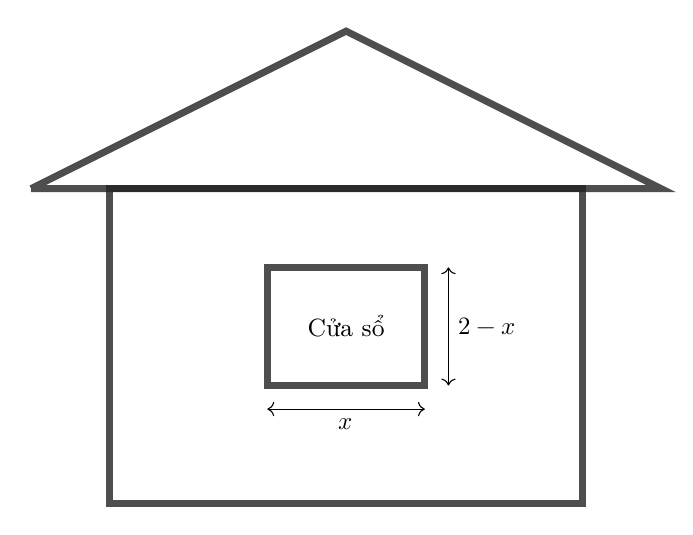
\begin{tikzpicture}[scale=1]

  % Nhà kho (hình chữ nhật + mái tam giác)
  \draw [line width=2.5pt, color=den-2, opacity=.8] (1,0) rectangle (7,4); 

  \draw [line width=2.5pt, color=den-2, opacity=.8] (0,4) -- (4,6) -- (8,4) -- (0,4); 

  % Cửa sổ hình chữ nhật
  \draw [smooth, line width=2.5pt, color=den-2, opacity=.8] (3,1.5) rectangle ++(2,1.5);

  \node at (4,2.25) {\small Cửa sổ};

  % Ghi chú chu vi
  \draw [<->] (5.3, 1.5) -- ++(0,1.5) node [midway,right] {\small $2-x$};

  \draw [<->] (3,1.2) -- ++(2,0) node [midway,below] {\small $x$};

\end{tikzpicture}

\end{document}
